A interação entre o ser humano e sua realidade tecnológica tem sido um tema de reflexão constante. Martin Heidegger, em "O Ser e o Tempo", propõe que nossa relação profunda com a tecnologia impacta de maneira determinante a qualidade de nossa experiência existencial  \cite{2012_Silva_DISSERTATION}. Observando o gesto quase instintivo de deslizar sobre uma tela sensível ao toque, é possível evidenciar esta perspectiva heideggeriana: à medida que dominamos tal interface, a fronteira entre humano e digital se torna menos perceptível, integrando nossa experiência no mundo digital de maneira mais orgânica. Complementarmente, O filósofo Merleau-Ponty, em sua análise fenomenológica do corpo, ressalta a centralidade do corpo como mediador em nossa relação com o mundo \cite{2011_MerleauPonty_BOOK}. Os dispositivos digitais contemporâneos, além de serem ferramentas, tornam-se extensões corpóreas, afetando diretamente como percebemos e nos conectamos com a realidade. Merleau-Ponty já destacava a maneira como objetos externos, como um chapéu que altera a altura de alguém, podem ser incorporados à nossa percepção corporal.

Esta compreensão fenomenológica encontra ecos em descobertas recentes nos campos da neurofisiologia e neuropsicologia. Por exemplo, o estudo de \citeonline{2004_Maravita} evidenciam que o uso de ferramentas modifica a representação neural do corpo em macacos, integrando-as ao 'esquema corporal'. Esse fenômeno pode sugerir uma adaptação cerebral à extensão sensorial proporcionada pela ferramenta, reforçando a ideia de que ferramentas e dispositivos como smartphones, além de influenciar nossos comportamentos através de mecanismos de recompensa, também reconfiguram nosso esquema corporal. Ao usar a câmera de um smartphone, por exemplo, nosso cérebro não só reconhece o dispositivo como uma ferramenta útil, mas também o integra como uma extensão dos nossos olhos, ampliando nossa capacidade de perceber e capturar o mundo ao nosso redor. Assim, a interação entre corpo e artefatos que o corpo produz, seja um chapéu, um martelo ou um smartphone, torna-se uma dança contínua de adaptação e reconfiguração.

\begin{figure}[ht]
	\centering
	\begin{subfigure}{0.45\textwidth}
		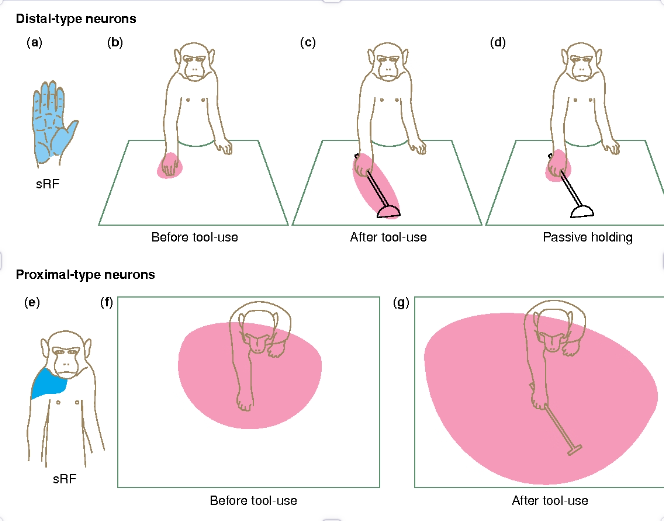
\includegraphics[width=\linewidth]{images/tools_for_the_body.png}
        \caption*{\citeonline{2004_Maravita}}
	\end{subfigure}
	\hfill
	\begin{subfigure}{0.45\textwidth}
		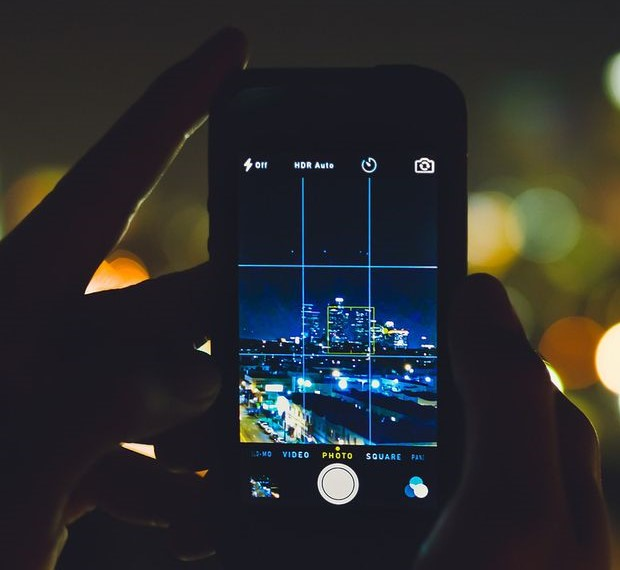
\includegraphics[width=\linewidth]{images/tools_for_the_mind.jpg}
		\caption*{Free-Photos/Pixabay}
	\end{subfigure}
	\caption{À esquerda, a extensão corpórea através da tecnologia é ilustrada pelo ajuste neural de macacos ao uso de ferramentas, um paralelo que ressoa com as teorias fenomenológicas sobre o corpo humano. À direita, a interação humana com o mundo digital, como um vislumbre pelo celular, reflete essa mesma interconexão entre o corpo e a tecnologia.}
\end{figure}

Ao considerarmos uma intersecção entre as ideias de Heidegger e o estudo contemporâneo dessas ferramentas tecnológicas, percebemos a relevância do conceito de Zuhandenheit, que descreve a tecnificação das mãos, ou seja, como as ferramentas se integram em nossas atividades cotidianas de forma fluida e transparente. No entanto, essa tecnificação excessiva das mãos em tempos contemporâneos pode levar à inautenticidade, à perda de uma conexão genuína com nosso ser e ao surgimento de um sentimento de ansiedade.

Em uma dimensão mais contemporânea, Pierre Lévy, em suas reflexões sobre o ciberespaço, destaca como a virtualização e a conectividade digital transformam a inteligência coletiva e a experiência social \cite{2010_Levy_BOOK}. O smartphone, neste contexto, não é apenas uma extensão do corpo, mas um portal para um espaço onde os indivíduos coletivamente constroem conhecimento e significado de forma paralela do que é considerado "vida real" mas com estímulos e formas de olhar adaptadas e interpretadas a partir das nossas experiências e vivências.

Contudo, esse entrelaçamento íntimo com a tecnologia traz consigo dilemas. Jacques Derrida, introduz o conceito de \textit{hauntologia}, o estado de assombração causado pela sensação de que o presente não corresponde às promessas do passado, alerta para um sentimento crescente de alienação no ciberespaço. 

Em um mundo onde a promessa era de conexões mais profundas e infinitas possibilidades, o que muitas vezes prevalece é uma sensação de deslocamento. A omnipresença de notificações e interações digitais em nossos smartphones, embora prometa autenticidade, pode, em muitos casos, entregar superficialidade. As preocupações de Heidegger sobre a inautenticidade se alinham com esta visão derridiana, e juntas, essas perspectivas lançam luz sobre os paradoxos da modernidade: enquanto a tecnologia se torna cada vez mais uma extensão de nós mesmos, nossa busca por conexões genuínas no mundo digital parece permanecer, em muitos aspectos, insatisfeita.

Embora as plataformas digitais de redes sociais tenham o potencial de aumentar o engajamento político e fomentar o diálogo, também são palco de um fenômeno preocupante: as câmaras de eco. Nas câmaras de eco, os usuários são expostos apenas a informações que confirmam suas crenças e tendências pré-existentes, contribuindo para a polarização das opiniões. Essa fragmentação das fontes de informação, descrita por Heidegger como uma forma de inautenticidade, e o fenômeno das bolhas de filtro, estudado por pesquisadores contemporâneos, compartilham características semelhantes e agravam o problema.

A inautenticidade, conceito central na filosofia de Heidegger, pode ser entendida como a falta de uma relação autêntica com o mundo e consigo mesmo. No contexto das plataformas de mídia social, a inautenticidade pode se manifestar quando os usuários adotam opiniões populares ou polêmicas para se encaixar em determinados grupos ou para ganhar aprovação e validação social. Essa busca por aceitação pode levar à polarização, à medida que as pessoas se alinham cada vez mais com visões extremas para se distinguir e ganhar reconhecimento dentro de suas comunidades online.

Essa tendência à inautenticidade é agravada pelos algoritmos das plataformas de mídia social, que personalizam o conteúdo exibido aos usuários com base em seu comportamento passado. Esses algoritmos, em busca de maximizar o engajamento e o tempo gasto nas plataformas, analisam o histórico de navegação, curtidas, compartilhamentos e interações do usuário para determinar quais conteúdos são mais propensos a serem do seu interesse. Como resultado, os usuários são apresentados principalmente a informações que se alinham com suas preferências e visões de mundo, enquanto conteúdos divergentes ou contraditórios são filtrados ou recebem menos destaque.

O processo de filtragem cria "bolhas" ao redor dos usuários, restringindo a variedade de informações a que são expostos. O estudo de \citeonline{2011_Pariser_BOOK} aponta que essas bolhas surgem de algoritmos que selecionam conteúdo baseado no histórico, conexões e preferências do usuário. Adicionalmente, \citeonline{2018_Aslay} enfatiza que a formação dessas bolhas não é determinada apenas pelos algoritmos, mas também pela interação do usuário com a plataforma, limitando sua exposição a diferentes perspectivas.

Um olhar sobre o TikTok, apresentado por \citeonline{2022_Boeker}, revela que sua bolha de filtragem considera diversos fatores, desde localização e idioma do usuário até tags dos vídeos e interações com o conteúdo. O algoritmo leva em conta não apenas preferências expressas, mas também análises de visão computacional e descrições associadas aos vídeos.

Em resumo, a formação de \textit{filter-bubbles} é um fenômeno multifacetado, influenciado tanto por algoritmos quanto pelo comportamento dos usuários. Essa interação molda a informação apresentada, limitando frequentemente a exposição a opiniões divergentes. Além disso, as plataformas sociais, por seu design e estrutura, muitas vezes incentivam comportamentos que reforçam essas bolhas. 

O artigo \citeonline{2022_Cross_PAGE} sugere que, a natureza dissociativa da internet e das plataformas sociais pode distorcer as boas intenções, fazendo com que os usuários se envolvam em comportamentos tóxicos, mesmo sem intenção maliciosa. O design das mídias sociais agita o tráfego de informações, em vez de acalmá-lo, muitas vezes tornando a toxicidade o caminho de menor resistência. Esta combinação de personalização algorítmica e a estrutura inherentemente dissociativa das redes sociais pode intensificar a formação e a profundidade das câmaras de eco.

É importante compreender e abordar o fenômeno das bolhas de filtro juntamente com as câmaras de eco, pois ambos têm implicações significativas para o discurso político e a democracia. A superação desses desafios requer esforços para aumentar a diversidade de perspectivas, garantir o acesso a informações diversas e promover a interação entre usuários com opiniões diferentes. Além disso, é fundamental que os usuários desenvolvam uma consciência crítica em relação à sua interação com as ferramentas tecnológicas, buscando uma relação autêntica com o mundo digital e evitando a dependência excessiva que pode levar à perda de contato com a realidade e à inautenticidade.

O impacto das câmaras de eco no discurso político é significativo. Estudos indicam que usuários expostos a uma maior diversidade de pontos de vista políticos têm maior probabilidade de se envolver em discussões políticas, enquanto aqueles expostos apenas a conteúdos similares aos seus têm menos probabilidade de engajar-se com notícias políticas. Essas câmaras de eco são particularmente acentuadas no Brasil, onde a polarização política tem aumentado desde 2010 \cite{2022_Ortellado}. É importante notar que pesquisas científicas sobre câmaras de eco frequentemente se concentraram na análise de redes sociais públicas, como Twitter, Facebook e Reddit. Diversas pesquisas têm investigado as dinâmicas das câmaras de eco nesses ambientes online. Por exemplo, estudos como o de \cite[p. 224]{2016_Vicario} examinaram o surgimento e a propagação de desinformação e polarização nas redes sociais, destacando a importância de entender esses fenômenos para a sociedade como um todo.

O Colab é uma plataforma brasileira de mídia social que visa promover a democracia participativa, permitindo que os usuários apresentem ideias e propostas para melhorar suas comunidades. Através do Colab, os cidadãos podem compartilhar problemas locais, sugerir soluções, colaborar com outros membros da comunidade e interagir com representantes governamentais. A plataforma tem sido elogiada por sua abordagem inovadora para o envolvimento cívico, incentivando uma participação mais ativa dos cidadãos na tomada de decisões e no aprimoramento de suas localidades. No entanto, assim como outras plataformas de mídia social, o Colab também enfrenta o desafio das câmaras de eco, onde os usuários tendem a seguir e interagir principalmente com aqueles que compartilham suas opiniões políticas, resultando em uma redução de perspectivas e uma possível erosão dos valores democráticos. Compreender as câmaras de eco no contexto do aplicativo Colab apresenta uma oportunidade valiosa de pesquisa considerando que muitas plataformas de mídia social não disponibilizam seus dados para acesso público, tornando desafiador o estudo das câmaras de eco em tais ambientes. Além de uma rede social, o Colab também oferece serviços de eGov. Empresas de eGov, ou governo eletrônico, são organizações que fornecem soluções digitais para apoiar o funcionamento e os serviços do governo. Elas se concentram em utilizar a tecnologia da informação e comunicação (TIC) para melhorar a eficiência, transparência e interação entre o governo e os cidadãos. Essas empresas oferecem uma variedade de serviços, como desenvolvimento de portais governamentais, plataformas de participação cidadã, sistemas de gestão de documentos, soluções de segurança digital, entre outros.

No ambiente atual de plataformas de mídia social e redes online, as interações digitais moldam percepções, opiniões e até mesmo comportamentos dos usuários. Nesse contexto, o aplicativo Colab se apresenta como um microcosmo dessas interações, oferece uma representação vívida de como as comunidades online se formam e operam. Assumindo um papel central nesta dissertação, o Colab é analisado através de um prisma de câmaras de eco, comunidades estreitamente conectadas em que crenças e opiniões semelhantes são reforçadas, muitas vezes excluindo perspectivas divergentes.

Sob esta perspectiva, são estabelecidas as seguintes suposições:

\begin{enumerate}
	\item Suposição 1: Usuários dentro do aplicativo Colab possuem personas discerníveis com base em seu comportamento e sentimentos expressos.
	\item Suposição 2: Usuários com personas similares podem formar conexões dentro da rede.
	\item Suposição 3: No contexto do Colab, as câmaras de eco se manifestam em comunidades fortemente interconectadas, que exibem comportamentos significativamente diferentes das demais partes da rede.
	\item Suposição 4: Se existirem, é provável que as câmaras de eco sejam significativamente isoladas da rede mais ampla, limitando a exposição a visões divergentes.
\end{enumerate}

Partindo dessas suposições, formulamos a seguinte hipótese central:

\begin{citacao}
	Se câmaras de eco existirem dentro das comunidades da rede do aplicativo Colab, é provável que estejam ligadas a usuários com interesses e comportamentos semelhantes, formando comunidades isoladas e estreitamente conectadas. Estas comunidades serviriam potencialmente como mecanismos de reforço para suas próprias crenças e opiniões, isolando-as ainda mais da rede geral.
\end{citacao}

Esta pesquisa é orientada pela seguinte questão principal:

\begin{citacao}
	Como um método heurístico quantitativo sintetizado pode ser efetivamente projetado e implementado para identificar e caracterizar câmaras de eco dentro da comunidade de rede do Colab?
\end{citacao}

Para abordar essa questão, a pesquisa será organizada em quatro etapas fundamentais:

\begin{enumerate}
	\item Análise exploratória da rede e interações dos usuários no Colab.
	\item Proposição de heurísticas para detecção de câmaras de eco.
	\item Investigação da formação de câmaras de eco por meio de simulações computacionais.
	\item Desenvolvimento de uma aplicação web para demonstrar as heurísticas de detecção de câmaras de eco e o treinamento de modelos de aprendizado de máquina para classificação de postagens.
\end{enumerate}

Este trabalho tem como objetivo examinar o fenômeno das câmaras de eco na plataforma de mídia social brasileira Colab, e propor estratégias para detecção desses fenômenos a partir de tecnicas de análise de redes. Utilizaremos o Gephi para uma primeira análise exploratória da rede e, posteriormente, Python e NetworkX para uma análise de redes mais aprofundada, focada em identificar câmaras de eco e seus nós principais. A modelagem baseada em agentes auxiliará na simulação de comportamentos e propagação de informações. Todas as análises e desenvolvimentos serão realizados no ambiente Google Colaboratory, favorecendo a reproducibilidade e colaboração.

Ao combinar os o arcabouço teórico da academia com os dados e experiência do Colab, é possível obter uma compreensão mais profunda das câmaras de eco em um contexto específico, isto é, uma rede social fomentada por interesses  de eGov. Isso não apenas aprimora nossa compreensão desses fenômenos sociais complexos, mas também fornece insights valiosos para o governo e aprimora as estratégias de engajamento cidadão nas cidades atendidas pelo Colab. Ao compreender melhor como essas câmaras influenciam as interações políticas e o diálogo cívico, o governo pode tomar medidas mais eficazes para combater a polarização, promover a diversidade de perspectivas e fortalecer a participação democrática. A pesquisa pode fornecer insights práticos que ajudarão o governo a tomar decisões informadas e a desenvolver estratégias eficientes para criar um ambiente político mais saudável e autêntico.

Além disso, os resultados deste estudo têm potencial para serem extrapolados e adaptados para outras plataformas de mídia social, contribuindo para um campo mais amplo de estudos sobre câmaras de eco e polarização online. Os insights obtidos também poderão guiar o Colab em futuras atualizações de seu sistema, incentivando maior diversidade e combatendo a formação de tais câmaras. Do ponto de vista acadêmico, a pesquisa é pioneira, aproveitando o acesso exclusivo aos dados do Colab para aprofundar nosso entendimento sobre um fenômeno que, em outras redes, permanece muitas vezes obscuro.